\subsection{Fase di progettazione di dettaglio e codifica}

\subsubsection{Incremento III}

I dati riportati di seguito si riferiscono al periodo che va dal 08-03-2021 al 10-03-2021.

\begin{minipage}[b]{0.65\linewidth}
\begin{small}
{
\setlength\arrayrulewidth{1.3pt}
\begin{longtable}{ c | c c c c c c | c} 
 \rowcolor{coloreRosso}
 \color{white}{\textbf{Nominativo}} &
 \color{white}{\textbf{RE}} &
 \color{white}{\textbf{AM}} &
 \color{white}{\textbf{AN}} &
 \color{white}{\textbf{PT}} &
 \color{white}{\textbf{PR}} &
 \color{white}{\textbf{VE}} &
 \color{white}{\textbf{Tot.}} \\
 	
 \BM{} & - & 3 & - & 2 & 4 & - & 9 \\ 
 \PA{} & - & - & - & - & 4 & 5 & 9 \\ 
 \RA{} & - & - & - & 6 & 1 & 3 & 10\\ 
 \SH{} & - & - & - & 1 & 5 & 3 & 9 \\ 
 \SG{} & - & - & - & 1 & 4 & 4 & 9 \\ 
 \SP{} & 2 & 2 & - & - & 4 & 2 & 10 \\ 
 \ZM{} & 2 & - & - & 3 & 1 & 3 & 9\\

 
 	\rowcolor{coloreRosso}
 	\color{white}{\textbf{Totale ore ruolo}} &
 	\color{white}{\textbf{4}} &
 	\color{white}{\textbf{5}} &
 	\color{white}{\textbf{-}} &
 	\color{white}{\textbf{13}} &
 	\color{white}{\textbf{23}} &
 	\color{white}{\textbf{20}} &
 	\color{white}{\textbf{65}} \\
	\rowcolor{white}
	\captionsetup{width=.9\textwidth}
 	\caption{Distribuzione delle ore nell'incremento III}
\end{longtable}
}
\end{small}
\end{minipage}
\begin{minipage}[b]{.3\linewidth}
\begin{small}
{
\setlength\arrayrulewidth{.7pt}
\begin{longtable}{ c | c | c} 
 	\rowcolor{coloreRosso}
 	\color{white}{\textbf{Ruolo}} &
 	\color{white}{\textbf{Ore}} &
 	\color{white}{\textbf{Costo €}} \\
 	
 	Responsabile & 4 & 120\\
 	Amministratore & 5 & 100\\
 	Analista & - & -\\
 	Progettista & 13 & 286\\
 	Programmatore & 23 & 345\\
 	Verificatore & 20 & 300\\
 	
 	\rowcolor{coloreRosso}
 	\color{white}{\textbf{Totale}} &
 	\color{white}{\textbf{65}} &
 	\color{white}{\textbf{1151 €}}\\
 	\rowcolor{white}
 	\caption{Costi per ruolo nell'incremento III}
\end{longtable}
}
\end{small}
\end{minipage}

\begin{figure}[!htb]   
    \centering
    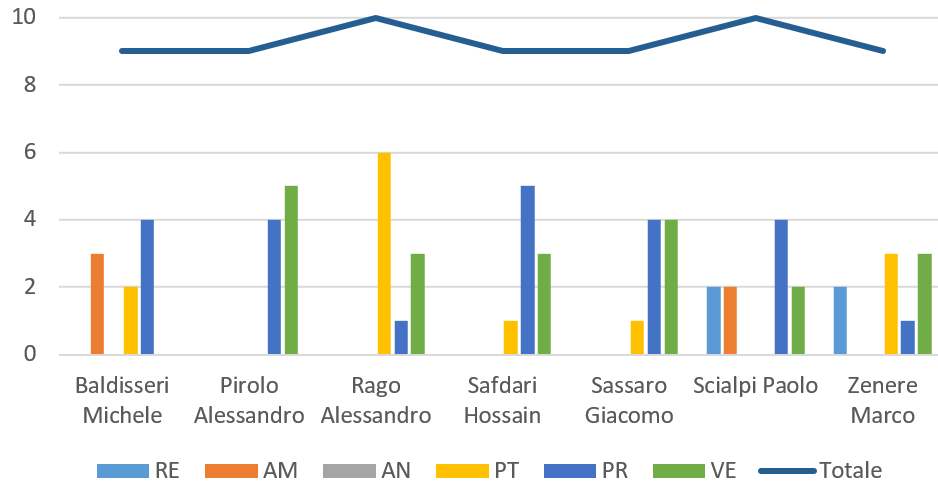
\includegraphics[width=0.95\textwidth]{Images/prev3}
	\caption{Ripartizione oraria per ciascun membro nell'incremento III}
\end{figure}





\subsubsection{Incremento IV}

I dati riportati di seguito si riferiscono al periodo che va dall' 10-03-2021 al 12-03-2021.

\begin{minipage}[b]{0.65\linewidth}
\begin{small}
{
\setlength\arrayrulewidth{1.3pt}
\begin{longtable}{ c | c c c c c c | c} 
 \rowcolor{coloreRosso}
 \color{white}{\textbf{Nominativo}} &
 \color{white}{\textbf{RE}} &
 \color{white}{\textbf{AM}} &
 \color{white}{\textbf{AN}} &
 \color{white}{\textbf{PT}} &
 \color{white}{\textbf{PR}} &
 \color{white}{\textbf{VE}} &
 \color{white}{\textbf{Tot.}} \\
 	
 \BM{} & - & 2 & - & 4 & 2 & 2 & 10 \\ 
 \PA{} & - & - & - & 5 & 6 & - & 11 \\ 
 \RA{} & - & - & - & 2 & 5 & 3 & 10\\ 
 \SH{} & - & - & - & 6 & 3 & 2 & 11 \\ 
 \SG{} & - & 2 & - & 6 & - & 2 & 10 \\ 
 \SP{} & 2 & - & - & - & 7 & 2 & 11 \\ 
 \ZM{} & 2 & 1 & - & - & 5 & 3 & 11 \\
 
 	\rowcolor{coloreRosso}
 	\color{white}{\textbf{Totale ore ruolo}} &
 	\color{white}{\textbf{4}} &
 	\color{white}{\textbf{5}} &
 	\color{white}{\textbf{-}} &
 	\color{white}{\textbf{23}} &
 	\color{white}{\textbf{28}} &
 	\color{white}{\textbf{14}} &
 	\color{white}{\textbf{74}} \\
	\rowcolor{white}
	\captionsetup{width=.9\textwidth}
 	\caption{Distribuzione delle ore nell'incremento IV}
\end{longtable}
}
\end{small}
\end{minipage}
\begin{minipage}[b]{.3\linewidth}
\begin{small}
{
\setlength\arrayrulewidth{.7pt}
\begin{longtable}{ c | c | c} 
 	\rowcolor{coloreRosso}
 	\color{white}{\textbf{Ruolo}} &
 	\color{white}{\textbf{Ore}} &
 	\color{white}{\textbf{Costo €}} \\
 	
 	Responsabile & 4 & 120\\
 	Amministratore & 5 & 100\\
 	Analista & - & -\\
 	Progettista & 23 & 506\\
 	Programmatore & 28 & 420\\
 	Verificatore & 14 & 210\\
 	
 	\rowcolor{coloreRosso}
 	\color{white}{\textbf{Totale}} &
 	\color{white}{\textbf{74}} &
 	\color{white}{\textbf{1356 €}}\\
 	\rowcolor{white}
 	\caption{Costi per ruolo nell'incremento IV}
\end{longtable}
}
\end{small}
\end{minipage}

\begin{figure}[!htb]   
    \centering
    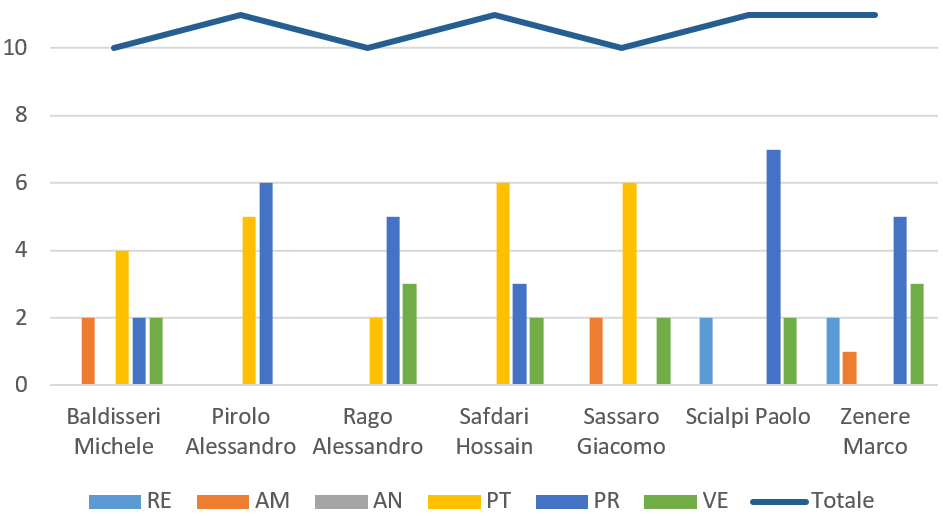
\includegraphics[width=0.95\textwidth]{Images/prev4}
	\caption{Ripartizione oraria per ciascun membro nell'incremento IV}
\end{figure}

\subsubsection{Incremento V}

I dati riportati di seguito si riferiscono al periodo che va dal 12-03-2021 al 16-03-2021.

\begin{minipage}[b]{0.65\linewidth}
\begin{small}
{
\setlength\arrayrulewidth{1.3pt}
\begin{longtable}{ c | c c c c c c | c} 
 \rowcolor{coloreRosso}
 \color{white}{\textbf{Nominativo}} &
 \color{white}{\textbf{RE}} &
 \color{white}{\textbf{AM}} &
 \color{white}{\textbf{AN}} &
 \color{white}{\textbf{PT}} &
 \color{white}{\textbf{PR}} &
 \color{white}{\textbf{VE}} &
 \color{white}{\textbf{Tot.}} \\
 	
 \BM{} & - & - & - & 5 & 3 & 2 & 10 \\ 
 \PA{} & - & 2 & - & 5 & - & 3 & 10 \\ 
 \RA{} & - & - & - & 2 & 7 & - & 9\\ 
 \SH{} & 2 & - & - & 1 & 5 & 2 & 10 \\ 
 \SG{} & - & 4 & - & 4 & - & 2 & 10\\ 
 \SP{} & - & - & - & 3 & 3 & 3 & 9 \\ 
 \ZM{} & 1 & - & - & - & 9 & - & 10 \\

 	\rowcolor{coloreRosso}
 	\color{white}{\textbf{Totale ore ruolo}} &
 	\color{white}{\textbf{3}} &
 	\color{white}{\textbf{6}} &
 	\color{white}{\textbf{-}} &
 	\color{white}{\textbf{20}} &
 	\color{white}{\textbf{27}} &
 	\color{white}{\textbf{12}} &
 	\color{white}{\textbf{68}} \\
	\rowcolor{white}
	\captionsetup{width=.9\textwidth}
 	\caption{Distribuzione delle ore nell'incremento V}
\end{longtable}
}
\end{small}
\end{minipage}
\begin{minipage}[b]{.3\linewidth}
\begin{small}
{
\setlength\arrayrulewidth{.7pt}
\begin{longtable}{ c | c | c} 
 	\rowcolor{coloreRosso}
 	\color{white}{\textbf{Ruolo}} &
 	\color{white}{\textbf{Ore}} &
 	\color{white}{\textbf{Costo €}} \\
 	
 	Responsabile & 3 & 90\\
 	Amministratore & 6 & 120\\
 	Analista & - & -\\
 	Progettista & 20 & 440\\
 	Programmatore & 27 & 405\\
 	Verificatore & 12& 180\\
 	
 	\rowcolor{coloreRosso}
 	\color{white}{\textbf{Totale}} &
 	\color{white}{\textbf{68}} &
 	\color{white}{\textbf{1235 €}}\\
 	\rowcolor{white}
 	\caption{Costi per ruolo nell'incremento V}
\end{longtable}
}
\end{small}
\end{minipage}

\begin{figure}[!htb]   
    \centering
    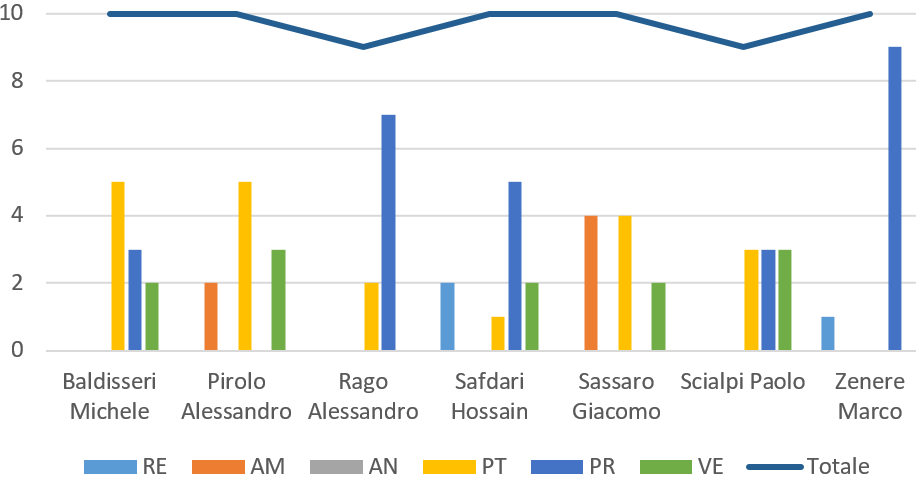
\includegraphics[width=.95\textwidth]{Images/prev5}
	\caption{Ripartizione oraria per ciascun membro nell'incremento V}
\end{figure}

\subsubsection{Incremento VI}

I dati riportati di seguito si riferiscono al periodo che va dal 16-03-2021 al 20-03-2021.

\begin{minipage}[b]{0.65\linewidth}
\begin{small}
{
\setlength\arrayrulewidth{1.3pt}
\begin{longtable}{ c | c c c c c c | c} 
 \rowcolor{coloreRosso}
 \color{white}{\textbf{Nominativo}} &
 \color{white}{\textbf{RE}} &
 \color{white}{\textbf{AM}} &
 \color{white}{\textbf{AN}} &
 \color{white}{\textbf{PT}} &
 \color{white}{\textbf{PR}} &
 \color{white}{\textbf{VE}} &
 \color{white}{\textbf{Tot.}} \\
 
 \BM{} & - & - & - & - & 8 & 2 & 10 \\ 
 \PA{} & - & 2 & - & - & 5 & 3 & 10 \\ 
 \RA{} & - & - & - & 5 & - & 5 & 10\\ 
 \SH{} & 2 & - & - & - & 5 & 2 & 9 \\ 
 \SG{} & - & - & - & 2 & 8 & - & 10 \\ 
 \SP{} & - & 3 & - & 2 & 5 & - & 10 \\ 
 \ZM{} & 1 & - & - & 2 & 2 & 4 & 9 \\
 
 	\rowcolor{coloreRosso}
 	\color{white}{\textbf{Totale ore ruolo}} &
 	\color{white}{\textbf{3}} &
 	\color{white}{\textbf{5}} &
 	\color{white}{\textbf{-}} &
 	\color{white}{\textbf{11}} &
 	\color{white}{\textbf{33}} &
 	\color{white}{\textbf{16}} &
 	\color{white}{\textbf{68}} \\
	\rowcolor{white}
	\captionsetup{width=.9\textwidth}
 	\caption{Distribuzione delle ore nell'incremento VI}
\end{longtable}
}
\end{small}
\end{minipage}
\begin{minipage}[b]{.3\linewidth}
\begin{small}
{
\setlength\arrayrulewidth{.7pt}
\begin{longtable}{ c | c | c} 
 	\rowcolor{coloreRosso}
 	\color{white}{\textbf{Ruolo}} &
 	\color{white}{\textbf{Ore}} &
 	\color{white}{\textbf{Costo €}} \\
 	
 	Responsabile & 3 & 60\\
 	Amministratore & 5 & 100\\
 	Analista & - & -\\
 	Progettista & 11 & 242\\
 	Programmatore & 33 & 495\\
 	Verificatore & 16 & 240\\
 	
 	\rowcolor{coloreRosso}
 	\color{white}{\textbf{Totale}} &
 	\color{white}{\textbf{68}} &
 	\color{white}{\textbf{1167 €}}\\
 	\rowcolor{white}
 	\caption{Costi per ruolo nell'incremento VI}
\end{longtable}
}
\end{small}
\end{minipage}

\begin{figure}[!htb]   
    \centering
    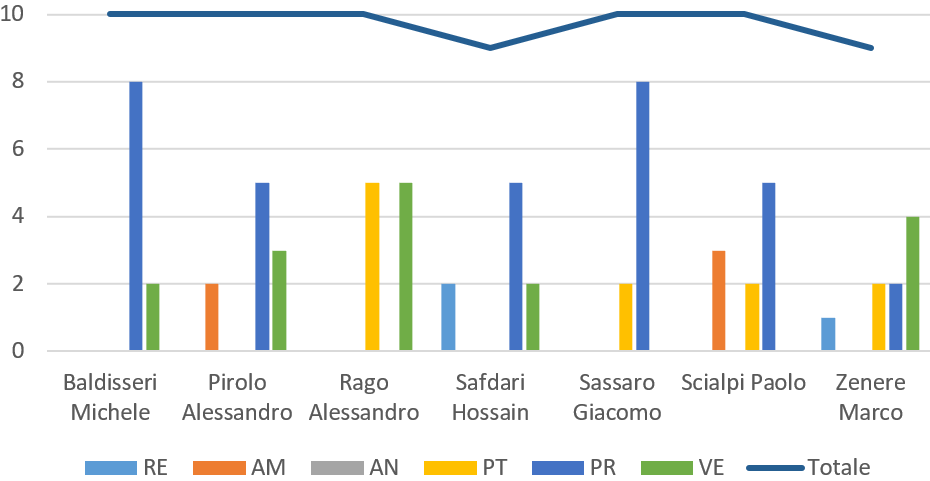
\includegraphics[width=0.95\textwidth]{Images/prev6}
	\caption{Ripartizione oraria per ciascun membro nell'incremento VI}
\end{figure}

\subsubsection{Incremento VII}

I dati riportati di seguito si riferiscono al periodo che va dal 20-03-2021 al 25-03-2021.

\begin{minipage}[b]{0.65\linewidth}
\begin{small}
{
\setlength\arrayrulewidth{1.3pt}
\begin{longtable}{ c | c c c c c c | c} 
 \rowcolor{coloreRosso}
 \color{white}{\textbf{Nominativo}} &
 \color{white}{\textbf{RE}} &
 \color{white}{\textbf{AM}} &
 \color{white}{\textbf{AN}} &
 \color{white}{\textbf{PT}} &
 \color{white}{\textbf{PR}} &
 \color{white}{\textbf{VE}} &
 \color{white}{\textbf{Tot.}} \\
 	
 \BM{} & - & - & - & - & 4 & 7 & 11 \\ 
 \PA{} & - & - & - & - & 8 & 2 & 10 \\ 
 \RA{} & 4 & - & - & - & 6 & 1 & 11\\ 
 \SH{} & 2 & 3 & - & - & 3 & 3 & 11 \\ 
 \SG{} & - & - & - & - & 9 & 2 & 11 \\ 
 \SP{} & - & - & - & 4 & 2 & 4 & 10 \\ 
 \ZM{} & - & 3 & - & 4 & 4 & - & 11 \\
 
 	\rowcolor{coloreRosso}
 	\color{white}{\textbf{Totale ore ruolo}} &
 	\color{white}{\textbf{6}} &
 	\color{white}{\textbf{6}} &
 	\color{white}{\textbf{-}} &
 	\color{white}{\textbf{8}} &
 	\color{white}{\textbf{36}} &
 	\color{white}{\textbf{19}} &
 	\color{white}{\textbf{75}} \\
	\rowcolor{white}
	\captionsetup{width=.9\textwidth}
 	\caption{Distribuzione delle ore nell'incremento VII}
\end{longtable}
}
\end{small}
\end{minipage}
\begin{minipage}[b]{.3\linewidth}
\begin{small}
{
\setlength\arrayrulewidth{.7pt}
\begin{longtable}{ c | c | c} 
 	\rowcolor{coloreRosso}
 	\color{white}{\textbf{Ruolo}} &
 	\color{white}{\textbf{Ore}} &
 	\color{white}{\textbf{Costo €}} \\
 	
 	Responsabile & 6 & 180\\
 	Amministratore & 6 & 120\\
 	Analista & - & -\\
 	Progettista & 8 & 176\\
 	Programmatore & 36 & 540\\
 	Verificatore & 19 & 285\\
 	
 	\rowcolor{coloreRosso}
 	\color{white}{\textbf{Totale}} &
 	\color{white}{\textbf{75}} &
 	\color{white}{\textbf{1301 €}}\\
 	\rowcolor{white}
 	\caption{Costi per ruolo nell'incremento VII}
\end{longtable}
}
\end{small}
\end{minipage}

\begin{figure}[!htb]   
    \centering
    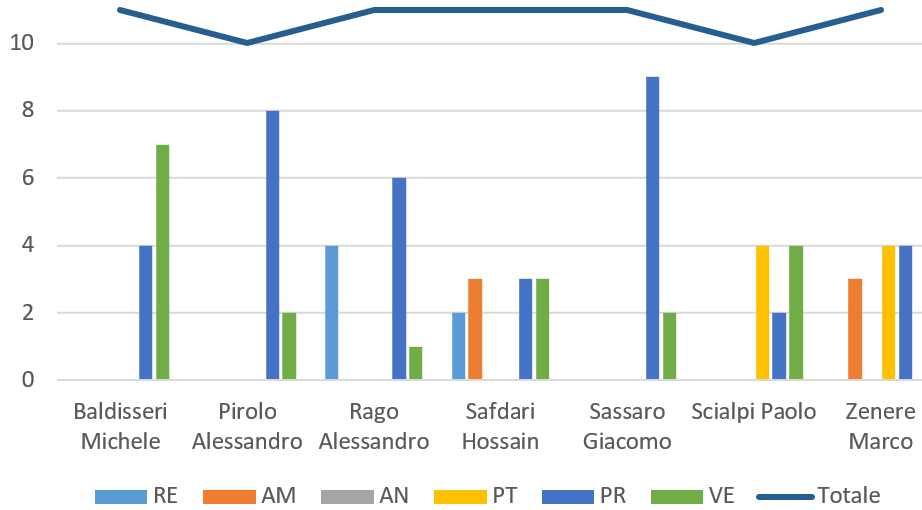
\includegraphics[width=0.95\textwidth]{Images/prev7}
	\caption{Ripartizione oraria per ciascun membro nell'incremento VII}
\end{figure}

\subsubsection{Riepilogo}

\begin{minipage}[b]{0.65\linewidth}
\begin{small}
{
\setlength\arrayrulewidth{1.3pt}
\begin{longtable}{ c | c c c c c c | c} 
 \rowcolor{coloreRosso}
 \color{white}{\textbf{Nominativo}} &
 \color{white}{\textbf{RE}} &
 \color{white}{\textbf{AM}} &
 \color{white}{\textbf{AN}} &
 \color{white}{\textbf{PT}} &
 \color{white}{\textbf{PR}} &
 \color{white}{\textbf{VE}} &
 \color{white}{\textbf{Tot.}} \\
 	
 \BM{} & - & 5 & - & 11 & 21 & 13 & 50 \\ 
 \SG{} & - & 6 & - & 13 & 21 & 10 & 50 \\ 
 \SH{} & 6 & 3 & - & 8 & 21 & 12 & 50 \\ 
 \PA{} & - & 4 & - & 10 & 21 & 15 & 50 \\ 
 \SP{} & 4 & 5 & - & 9 & 21 & 11 & 50 \\ 
 \RA{} & 4 & - & - & 15 & 21 & 10 & 50 \\ 
 \ZM{} & 6 & 4 & - & 9 & 21 & 10 & 50 \\
 
 \rowcolor{coloreRosso}
 	\color{white}{\textbf{Totale ore ruolo}} &
 	\color{white}{\textbf{20}} &
 	\color{white}{\textbf{27}} &
 	\color{white}{\textbf{-}} &
 	\color{white}{\textbf{75}} &
 	\color{white}{\textbf{147}} &
 	\color{white}{\textbf{81}} &
 	\color{white}{\textbf{350}} \\
 \rowcolor{white}
 \captionsetup{width=.9\textwidth}
 \caption{Distribuizione delle ore nel periodo di Progettazione di dettaglio e Codifica}
\end{longtable}
}
\end{small}
\end{minipage}
\begin{minipage}[b]{.3\linewidth}
\begin{small}
{
\setlength\arrayrulewidth{.7pt}
\begin{longtable}{ c | c | c} 
 	\rowcolor{coloreRosso}
 	\color{white}{\textbf{Ruolo}} &
 	\color{white}{\textbf{Ore}} &
 	\color{white}{\textbf{Costo €}} \\
 	
 	Responsabile & 20 & 600\\
 	Amministratore & 27 & 540\\
 	Analista & - & -\\
 	Progettista & 75 & 1650\\
 	Programmatore & 147 & 2205\\
 	Verificatore & 81 & 1215\\
 	
 	\rowcolor{coloreRosso}
 	\color{white}{\textbf{Totale}} &
 	\color{white}{\textbf{350}} &
 	\color{white}{\textbf{6210 €}}\\
 	\rowcolor{white}
 	\caption{Costi per ruolo nel periodo di Prog. di dettaglio e Codifica}
\end{longtable}
}
\end{small}
\end{minipage}

I seguenti grafici riassumo i dati ottenuti.

\begin{figure}[!htb]
   \begin{minipage}{0.6\textwidth}
     \centering
     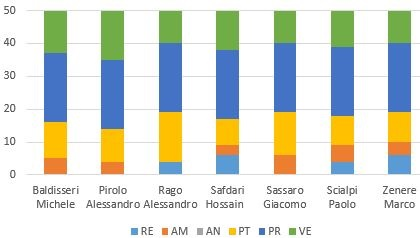
\includegraphics{Images/PO-Codifica}
     \caption{Ripartizione oraria per ciascun membro nella fase di Prog. di dettaglio e Codifica}
   \end{minipage}\hspace{0.1\textwidth}
   \begin{minipage}{0.3\textwidth}
     \centering
     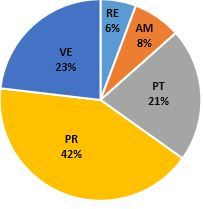
\includegraphics[width=.9\textwidth]{Images/PE-Codifica}
     \captionsetup{width=1.1\textwidth}
     \caption{Ripartizione ore totali nella fase di Prog. di dettaglio e Codifica}
   \end{minipage}
\end{figure}

\newpage